\documentclass[10pt]{article}

\usepackage{color,times,graphicx,epstopdf,fancyhdr,amsfonts,amsthm,amsmath,algorithm,algorithmic,xspace,hyperref}
\usepackage[left=1in,top=1in,right=1in,bottom=1in]{geometry}
\usepackage{sect sty}	%For centering section headings
\usepackage{enumerate}	%Allows more labeling options for enumerate environments
\usepackage{epsfig}
\usepackage[space]{grffile}
\usepackage{booktabs}

% This will set LaTeX to look for figures in the same directory as the .tex file
\graphicspath{.} % The dot means current directory.

\pagestyle{fancy}

\lhead{\YOURID}
\chead{Square Root List}
\rhead{\today}
\lfoot{Williams College}
\cfoot{\thepage}
\rfoot{Fall 2020}

% Some commands for changing header and footer format
\renewcommand{\headrulewidth}{0.4pt}
\renewcommand{\headwidth}{\textwidth}
\renewcommand{\footrulewidth}{0.4pt}
\newcommand{\nonterm}[1]{$\langle$#1$\rangle$}

% These let you use common environments
\newtheorem{claim}{Claim}
\newtheorem{definition}{Definition}
\newtheorem{theorem}{Theorem}
\newtheorem{lemma}{Lemma}
\newtheorem{observation}{Observation}
\newtheorem{question}{Question}

\setlength{\parindent}{0cm}

\setlength{\columnseprule}{0.1pt}
\def\columnseprulecolor{\color{black}}


% Edit below as instructed
\newcommand{\YOURID}{Petros Markopoulos}
\newcommand{\ProblemHeader}

\begin{document}

\vspace{\baselineskip}	% Add some vertical space

\section{Introduction}
\subsection{What is a Linked List}
A Linked List is a simple data structure consisting of what is usually referred to as \textit{Nodes}. A Node contains some piece of data as well as a pointer to the next node (it can also contain a pointer to the previous node, to create a Doubly Linked List, which is actually what is used in the implementation of SqrtList). Thus, the whole list can be accessed by starting at the first node (usually referred to as the \textit{head}) and following the pointers until the end of the list (\textit{tail}) is reached. A Linked List does not have random access, and thus although given a specific node all operations (inserting a new node next to it, removing the node, getting its value or setting its value) are done in $O(1)$ time, doing the same operations given an \textit{index} instead of a node are all done in $O(n)$ time (where $n$ is the length of the list), as, in the worst case, the entire list needs to be traveresed to access the node at that index and perform the operation.

\begin{figure}[hbp]
	\centering
	\textbf{A Singly Linked List}\par\medskip
	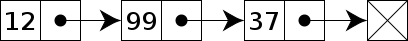
\includegraphics[width=.5\textwidth]{./img/singly_linked_list.png}
\end{figure}
\begin{figure}[hbp]
	\centering
	\textbf{A Doubly Linked List}\par\medskip
	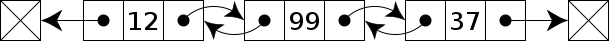
\includegraphics[width=.5\textwidth]{./img/doubly_linked_list.png}
\end{figure}
\subsection{What is the Square Root List}
The \textit{Square Root List} is an idea I had after examining Linked Lists in my Data Structures class and it is an attempt to improve on the runtime of the aforementioned operations by storing some extra pointers along with the real list. A second list is maintained, which stores pointers for about every $\sqrt{n}$ elements of the main list, where $n$ is the length of the main list. When an element of the main list needs to be accessed, instead of traversing the main list directly, the secondary list is traversed instead, thus "skipping" over many elements. When a point close to the desired element has been reached, the traversal of the main list starts and the element is reached. We will show later that this traversal is done in $O(\sqrt{n})$ time.
\begin{figure}[hbp]
	\centering
	\textbf{A Square Root List}\par\medskip
	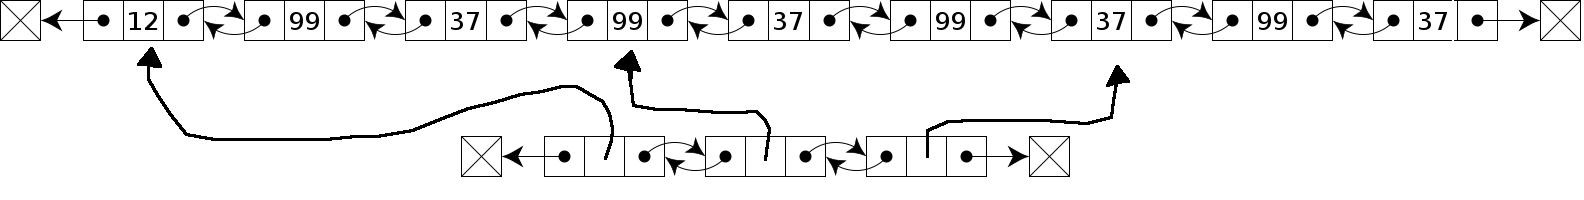
\includegraphics[width=.7\textwidth]{./img/square_root_list.png}
\end{figure}
\section{Operation Runtime for the Square Root List}
\subsection{Notes}
Before showing that the runtime is indeed what was claimed before, a point needs to be clarified. I said that the secondary list is about $\sqrt{n}$ elements long. That "about" means the following: because add and remove operations are contantly changing the length $n$ of the list, instead of constantly keeping up with those changes, the list uses another number $m$ as a stand-in for the length of the list. $m$ is updated in the buildMeta() method of the class, where it is set to be equal to the real size of the list. buildMeta is only called when the size of the list has diverged too much from the value of $m$. When an insertion happens but the threshold for calling buildMeta is not surpassed, then retreat is called. retreat traverses the secondary list from the site of the insertion until the end and updates each stored node to be equal to its next node. This ensures that the chunks between two stored nodes remain equally sized and that the list works correctly. Similarly, when a removal happens, advance is called which works identically to retreat, but updates nodes to be their previous node instead of their next.
\subsection{Proofs}
Claim: $\sqrt{m}$ is bounded by $O(\sqrt{n})$.
\begin{proof}
	$ $\\
	We can see from the code that $m - \sqrt{m} \leq n \leq m + \sqrt{m}$, since when either of those bounds is exceeded, buildMeta is called and then $m = n$.\\
	$m - \sqrt{m} \leq n \iff m - \sqrt{m} - n \leq 0$ (inequality (1))\\
	By setting $x = \sqrt{m}$ inequality (1) becomes $x^2 - x - n \leq 0$ (inequality (2))\\
	$x^2 - x - n = 0 \iff x = \frac{1 + \sqrt{1 + 4n}}{2} \; or \; x = \frac{1 - \sqrt{1 + 4n}}{2}$\\
	Therefore inequality (2) is satisfied by $\frac{1 - \sqrt{1 + 4n}}{2} \leq x \leq \frac{1 + \sqrt{1 + 4n}}{2}$.\\
	This gives us that $0 \leq \sqrt{m} \leq \frac{1 + \sqrt{1 + 4n}}{2}$.\\
	$\sqrt{m} \leq \frac{1}{2} + \frac{\sqrt{1 + 4n}}{2} \leq \frac{\sqrt{n}}{2} + \frac{\sqrt{5n}}{2}$\\
	Thus $\sqrt{m} \leq \frac{\sqrt{5} + 1}{2}\sqrt{n}$ and therefore $\sqrt{m}$ is bounded by $O(\sqrt{n})$.

\end{proof}

Claim: The getNode(idx) method works in $O(\sqrt{n})$ time.
\begin{proof}
	$ $\\
	In the worst case, getNode has to traverse the entire secondary list to find the node closest to the desired index. The length of the secondary list is, by its construction $\sqrt{m}$. Then, another traversal is needed, from the node stored in the secondary list up to the desired index. That traversal also has at most $\sqrt{m}$ nodes, since, the secondary list stores one node every $\sqrt{m}$ nodes. Thus, the entire traversal is at most $2\sqrt{m} - 1$ nodes long, which means that it is bounded by $O(\sqrt{m})$ and thus $O(\sqrt{n})$.
\end{proof}

Claim: The get(idx) method works in $O(\sqrt{n})$ time.
\begin{proof}
	$ $\\
	The method consists of a single call to getNode(idx)a field access. Since getNode(idx) works in $O(\sqrt{n})$ time, this method does too.
\end{proof}

Claim: The set(idx) method works in $O(\sqrt{n})$ time.
\begin{proof}
	$ $\\
	The method consists of a single call to getNode(idx) and a value update. Since getNode(idx) works in $O(\sqrt{n})$ time, this method does too.
\end{proof}

Claim: The insert(val, idx) method works in amortized $O(\sqrt{n})$ time.
\begin{proof}
	$ $\\
	The method calls getNode(idx) which is $O(\sqrt{n})$ and then creates a new node (which takes constant time with respect to the length of the list).\\
	In every call it will make a call to retreat(inseartionIdx), which traverses the entire secondary list and thus takes $O(\sqrt{m})$ time.\\
	Once every $\sqrt{m}$ calls it will make a call to $buildMeta()$ which traverses the entire main list so it takes $O(n)$ time. Distributing the cost of that call over the $\sqrt{m}$ calls yields $O(\frac{n}{\sqrt{m}})$ time.\\
	Therefore, overall, insert(val, idx) runs in $O(\sqrt{n}) + O(\sqrt{m}) + O(\frac{n}{\sqrt{m}})$ time, which is bounded by $O(\sqrt{n})$.
\end{proof}

Claim: The remove(idx) method works in amortized $O(\sqrt{n})$ time.
\begin{proof}
	$ $\\
	This method works identically with the insert(val, idx) method, and therefore has the same runtime.
\end{proof}

\end{document}
